\documentclass[a4paper,12pt]{article}
\usepackage[utf8]{inputenc}
\usepackage[T2A]{fontenc}
\usepackage[english, russian]{babel}
\usepackage{titlesec}
\titleformat{\section}{\normalfont\Large\bfseries}{\thesection.}{1em}{}
\titleformat{\subsection}{\normalfont\large\bfseries}{\thesubsection.}{1em}{}
\usepackage{tocloft}
\renewcommand{\cftsecleader}{\cftdotfill{\cftdotsep}}
\usepackage{hyperref}
\usepackage{geometry}
\geometry{top=2cm, bottom=2cm, left=2cm, right=2cm}
\setlength{\parindent}{1.25cm}
\setlength{\parskip}{0pt}
\usepackage{amsmath,amssymb}
\usepackage{listings}
\usepackage{xcolor}
\usepackage{graphicx}
\hypersetup{hidelinks}
\hypersetup{pageanchor=false}

\definecolor{background}{RGB}{255, 255, 255}  % Белый фон
\definecolor{keywords}{RGB}{0, 0, 255}        % Синий для ключевых слов
\definecolor{comments}{RGB}{0, 128, 0}        % Зелёный для комментариев
\definecolor{strings}{RGB}{163, 21, 21}       % Красный для строк
\definecolor{numbers}{RGB}{100, 200, 100}       % Фиолетовый для чисел
\definecolor{identifiers}{RGB}{0, 0, 0}       % Чёрный для идентификаторов

\lstdefinestyle{mystyle}{
    backgroundcolor=\color{background},   
    commentstyle=\color{comments},
    keywordstyle=\color{keywords},
    numberstyle=\tiny\color{numbers},
    stringstyle=\color{strings},
    basicstyle=\ttfamily\footnotesize\color{identifiers},
    breakatwhitespace=false,         
    breaklines=true,                 
    captionpos=b,                    
    keepspaces=true,                 
    numbers=left,                    
    numbersep=5pt,                  
    showspaces=false,                
    showstringspaces=false,
    showtabs=false,                  
    tabsize=2,
    language=C++
}

\lstset{style=mystyle}

\begin{document}
\begin{titlepage}
\begin{center}
\textbf{МИНИСТЕРСТВО НАУКИ И ВЫСШЕГО ОБРАЗОВАНИЯ РОССИЙСКОЙ ФЕДЕРАЦИИ} \\
\textbf{Федеральное государственное автономное образовательное учреждение высшего образования} \\
\textbf{«Национальный исследовательский Нижегородский государственный университет им. Н.И. Лобачевского»} \\[1cm]
\textbf{Институт информационных технологий, математики и механики }\\[0.5cm]
\textbf{Кафедра: Математического обеспечения и суперкомпьютерных технологий}\\[0.5cm]
Направление подготовки: «Программная инженерия»\\
Профиль подготовки: «Общий»\\

\vfill

Отчёт по лабораторной работе на тему:\\
{\Large
\textbf{«Быстрая сортировка с простым слиянием»} \\
}
\vfill
\begin{flushright}
\textbf{Выполнил}:\\
студент группы 3822Б1ПР2 \\
Варфоломеев Григорий \\
\vspace{1cm}
\textbf{Преподаватель}: \\
Сысоев Александр Владимирович \\
\textbf{Руководители}: \\
Нестеров Александр Юрьевич\\
Оболенский Арсений Андреевич\\
\end{flushright}
\vfill
Нижний Новгород \\
2024
\end{center}
\end{titlepage}

\tableofcontents
\newpage

\section{Введение}
В данном отчёте рассматривается задача реализации быстрой сортировки с простым слиянием. Основная цель работы — разработать эффективный алгоритм сортировки, который может быть распараллелен с использованием модели MPI (Message Passing Interface). Быстрая сортировка — это алгоритм, основанный на принципе «разделяй и властвуй», который разбивает массив на подмассивы, сортирует их рекурсивно и объединяет результаты. Параллельная реализация позволяет ускорить процесс сортировки за счёт распределения данных между несколькими процессами.

\section{Постановка задачи}
В рамках данной работы необходимо:
\begin{enumerate}
    \item Реализовать последовательную версию быстрой сортировки с простым слиянием.
    \item Разработать параллельную версию алгоритма с использованием MPI.
    \item Провести валидацию корректности работы алгоритма (сравнение с последовательной реализацией).
    \item Проанализировать производительность последовательной и параллельной версий на различных объёмах данных.
\end{enumerate}

\section{Описание алгоритма}
Быстрая сортировка — это алгоритм сортировки, который работает по принципу «разделяй и властвуй». Основные шаги алгоритма:
\begin{enumerate}
    \item Выбор опорного элемента (pivot) из массива.
    \item Разделение массива на две части: элементы, меньшие опорного, и элементы, большие опорного.
    \item Рекурсивное применение алгоритма к каждой из частей.
    \item Объединение отсортированных частей в один массив.
\end{enumerate}

В параллельной реализации данные распределяются между процессами. Каждый процесс выполняет локальную сортировку своей части данных, а затем отправляет результаты корневому процессу. Корневой процесс объединяет отсортированные части в окончательный результат.

\section{Схема распараллеливания}
Параллельная реализация быстрой сортировки с использованием MPI включает следующие шаги:
\begin{enumerate}
    \item \textbf{Распределение данных}: Корневой процесс (rank = 0) распределяет данные между всеми процессами.
    \item \textbf{Локальная сортировка}: Каждый процесс выполняет быструю сортировку на своей части данных.
    \item \textbf{Сбор результатов}: Каждый процесс отправляет отсортированные данные корневому процессу.
    \item \textbf{Объединение результатов}: Корневой процесс объединяет отсортированные части в один массив.
\end{enumerate}

\section{Результаты экспериментов}
Для оценки производительности последовательной и параллельной версий алгоритма использовалась следующая тестовая система:
\begin{itemize}
    \item OS: Windows 10 Pro ver.22H2
    \item CPU: 13th Gen Intel(R) Core(TM) i7-13700K   3.40 GHz
    \item RAM: 32,0 GB
\end{itemize}

На основе выполнения тестов для параллельной версии (на 2, 3, 4, 6, 8, 10 и 12 процессах) была создана следующая таблица:

\begin{tabular}{|c|c|c|c|}
    \hline
    Число процессов & Вид теста      & Время выполнения (с) & Ускорение \\ \hline
    1               & pipeline\_run & 1.163               & 1      \\ \hline
    1               & task\_run     & 1.24                & 1      \\ \hline
    2               & pipeline\_run & 1.560                & 0.745513      \\ \hline
    2               & task\_run     & 1.666                & 0.744298      \\ \hline
    3               & pipeline\_run & 0.490                & 2.373469      \\ \hline
    3               & task\_run     & 0.514                & 2.412451      \\ \hline
    4               & pipeline\_run & 0.420               & 2.769048     \\ \hline
    4               & task\_run     & 0.453                & 2.737308      \\ \hline
    6              & pipeline\_run & 0.311                & 3.739550      \\ \hline
    6              & task\_run     & 0.325                & 3.815385      \\ \hline
    8              & pipeline\_run & 0.424                & 2.742925      \\ \hline
    8              & task\_run     & 0.453                & 2.737308      \\ \hline
    10              & pipeline\_run & 0.367                & 3.168937      \\ \hline
    10              & task\_run     & 0.382                & 3.246073      \\ \hline
    12              & pipeline\_run & 0.326                & 3.567485      \\ \hline
    12              & task\_run     & 0.353                & 3.512748      \\ \hline
\end{tabular}

\subsection{График зависимости времени выполнения от числа процессов}
\begin{center}
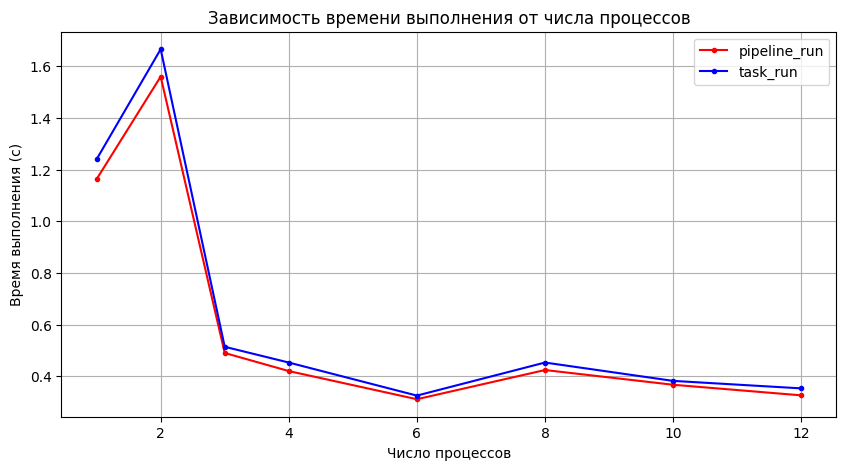
\includegraphics[width=0.8\textwidth]{images/time num.png}
\end{center}

\subsection{График зависимости ускорения от числа процессов}
\begin{center}
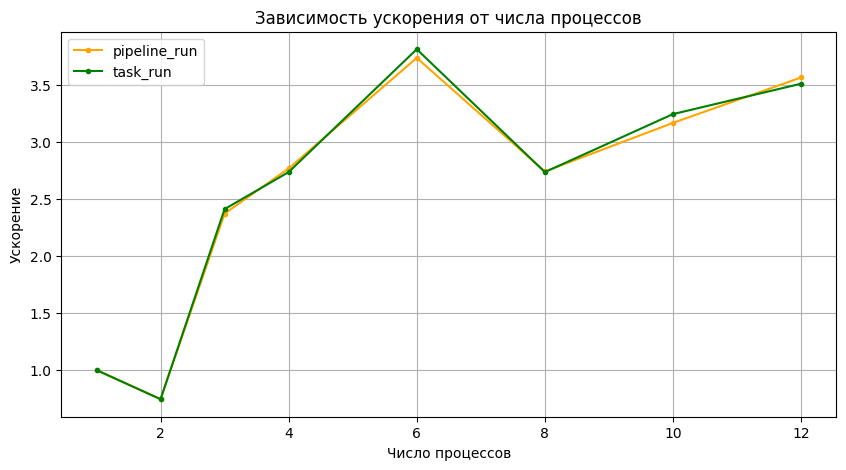
\includegraphics[width=0.8\textwidth]{images/speed num.png}
\end{center}

\subsection{График зависимости времени выполнения от количества элементов на 4 процессах}
\begin{center}
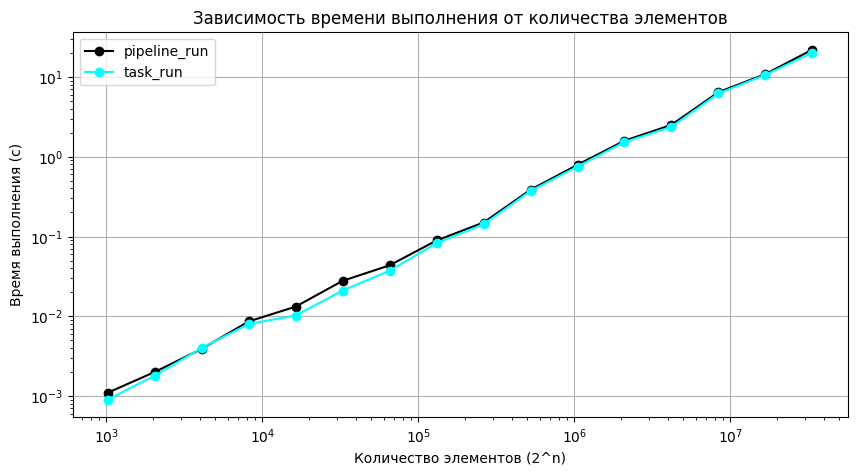
\includegraphics[width=0.8\textwidth]{images/time els four processes.png}
\end{center}

\newpage

\section{Заключение}
В ходе работы была реализована последовательная и параллельная версии быстрой сортировки с простым слиянием. Параллельная реализация показала значительное ускорение по сравнению с последовательной версией, особенно при увеличении числа процессов. Это подтверждает эффективность использования MPI для распараллеливания алгоритмов сортировки.

Основные направления улучшения:
\begin{itemize}
    \item Оптимизация процесса слияния данных на корневом процессе.
    \item Использование более сложных схем распределения данных для уменьшения накладных расходов.
\end{itemize}

\newpage

\section{Приложение}

\subsection{ops\_seq.hpp}
\begin{lstlisting}[language=C++]
#pragma once

#include <string>
#include <vector>

#include "core/task/include/task.hpp"

namespace varfolomeev_g_quick_sort_simple_merge_seq {

class TestTaskSequential : public ppc::core::Task {
 public:
  explicit TestTaskSequential(std::shared_ptr<ppc::core::TaskData> taskData_) : Task(std::move(taskData_)) {}
  bool pre_processing() override;
  bool validation() override;
  bool run() override;
  bool post_processing() override;

  static void quickSort(std::vector<int>& vec) { quickSortRecursive(vec, 0, vec.size() - 1); }

 private:
  static void quickSortRecursive(std::vector<int>& vec, int left, int right) {
    if (left >= right) return;
    int p = vec[(left + right) / 2];
    int i = left;
    int j = right;
    while (i <= j) {
      while (vec[i] < p) i++;
      while (vec[j] > p) j--;
      if (i <= j) {
        std::swap(vec[i], vec[j]);
        i++;
        j--;
      }
    }
    quickSortRecursive(vec, left, j);
    quickSortRecursive(vec, i, right);
  }

  std::vector<int> input_;
  std::vector<int> res;
};

}  // namespace varfolomeev_g_quick_sort_simple_merge_seq
\end{lstlisting}

\subsection{ops\_seq.cpp}
\begin{lstlisting}[language=C++]
#include "seq/varfolomeev_g_quick_sort_simple_merge/include/ops_seq.hpp"

bool varfolomeev_g_quick_sort_simple_merge_seq::TestTaskSequential::pre_processing() {
  internal_order_test();
  input_ = std::vector<int>(taskData->inputs_count[0]);
  auto* tmp_ptr = reinterpret_cast<int*>(taskData->inputs[0]);
  for (unsigned i = 0; i < taskData->inputs_count[0]; i++) {
    input_[i] = tmp_ptr[i];
  }
  res = input_;
  return true;
}

bool varfolomeev_g_quick_sort_simple_merge_seq::TestTaskSequential::validation() {
  internal_order_test();
  return (taskData->outputs_count.size() == 1 && taskData->inputs_count.size() == 1 && taskData->inputs_count[0] > 0 &&
          taskData->inputs_count[0] == taskData->outputs_count[0]);
}

bool varfolomeev_g_quick_sort_simple_merge_seq::TestTaskSequential::run() {
  internal_order_test();
  quickSort(res);
  return true;
}

bool varfolomeev_g_quick_sort_simple_merge_seq::TestTaskSequential::post_processing() {
  internal_order_test();
  auto* output_ptr = reinterpret_cast<int*>(taskData->outputs[0]);
  std::copy(res.begin(), res.end(), output_ptr);
  return true;
}
\end{lstlisting}

\subsection{ops\_mpi.hpp}
\begin{lstlisting}[language=C++]
#pragma once

#include <gtest/gtest.h>

#include <boost/mpi/collectives.hpp>
#include <boost/mpi/communicator.hpp>
#include <memory>
#include <numeric>
#include <utility>
#include <vector>

#include "core/task/include/task.hpp"

namespace varfolomeev_g_quick_sort_simple_merge_mpi {

class TestTaskSequential : public ppc::core::Task {
 public:
  explicit TestTaskSequential(std::shared_ptr<ppc::core::TaskData> taskData_) : Task(std::move(taskData_)) {}
  bool pre_processing() override;
  bool validation() override;
  bool run() override;
  bool post_processing() override;

  static void quickSort(std::vector<int>& vec) { quickSortRecursive(vec, 0, vec.size() - 1); }

 private:
  // main realization
  static void quickSortRecursive(std::vector<int>& vec, int left, int right) {
    if (left >= right) return;
    int p = vec[(left + right) / 2];
    int i = left;
    int j = right;
    while (i <= j) {
      while (vec[i] < p) i++;
      while (vec[j] > p) j--;
      if (i <= j) {
        std::swap(vec[i], vec[j]);
        i++;
        j--;
      }
    }
    quickSortRecursive(vec, left, j);
    quickSortRecursive(vec, i, right);
  }

  std::vector<int> input_;
  std::vector<int> res;
};

class TestMPITaskParallel : public ppc::core::Task {
 public:
  explicit TestMPITaskParallel(std::shared_ptr<ppc::core::TaskData> taskData_) : Task(std::move(taskData_)) {}

  bool pre_processing() override;
  bool validation() override;
  bool run() override;
  bool post_processing() override;

 private:
  std::vector<int> input_, local_input_;
  std::vector<int> res;
  boost::mpi::communicator world;

  static std::vector<int> quickSortRecursive(const std::vector<int>& vec) {
    if (static_cast<int>(vec.size()) <= 1) {
      return vec;
    }

    int p = vec[static_cast<int>(vec.size()) / 2];

    std::vector<int> left;
    std::vector<int> right;
    std::vector<int> equal;
    for (int i = 0; i < static_cast<int>(vec.size()); ++i) {
      if (vec[i] < p) {
        left.emplace_back(vec[i]);
      }
      if (vec[i] > p) {
        right.emplace_back(vec[i]);
      }
      if (vec[i] == p) {
        equal.emplace_back(vec[i]);
      }
    }
    std::vector<int> resLeft = quickSortRecursive(left);
    std::vector<int> resRight = quickSortRecursive(right);

    std::vector<int> mergeEqualRight = merge(equal, resRight);
    return merge(resLeft, mergeEqualRight);
  }

  static std::vector<int> merge(const std::vector<int>& vec1, const std::vector<int>& vec2) {
    std::vector<int> mergedvec;
    mergedvec.reserve(vec1.size() + vec2.size());
    int i = 0;
    int j = 0;
    while (i < static_cast<int>(vec1.size()) && j < static_cast<int>(vec2.size())) {
      if (vec1[i] < vec2[j]) {
        mergedvec.push_back(vec1[i++]);
      } else {
        mergedvec.push_back(vec2[j++]);
      }
    }

    mergedvec.insert(mergedvec.end(), vec1.begin() + i, vec1.end());
    mergedvec.insert(mergedvec.end(), vec2.begin() + j, vec2.end());

    return mergedvec;
  }
};

}  // namespace varfolomeev_g_quick_sort_simple_merge_mpi

\end{lstlisting}

\subsection{ops\_mpi.cpp}
\begin{lstlisting}[language=C++]
#include "mpi/varfolomeev_g_quick_sort_simple_merge/include/ops_mpi.hpp"

#include <boost/mpi.hpp>
#include <boost/serialization/vector.hpp>
#include <vector>

bool varfolomeev_g_quick_sort_simple_merge_mpi::TestTaskSequential::pre_processing() {
  internal_order_test();
  input_ = std::vector<int>(taskData->inputs_count[0]);
  auto* tmp_ptr = reinterpret_cast<int*>(taskData->inputs[0]);
  for (unsigned i = 0; i < taskData->inputs_count[0]; i++) {
    input_[i] = tmp_ptr[i];
  }
  res = input_;
  return true;
}

bool varfolomeev_g_quick_sort_simple_merge_mpi::TestTaskSequential::validation() {
  internal_order_test();
  return taskData->outputs_count.size() == 1 && taskData->inputs_count.size() == 1;
}

bool varfolomeev_g_quick_sort_simple_merge_mpi::TestTaskSequential::run() {
  internal_order_test();
  quickSort(res);
  return true;
}

bool varfolomeev_g_quick_sort_simple_merge_mpi::TestTaskSequential::post_processing() {
  internal_order_test();
  auto* output_ptr = reinterpret_cast<int*>(taskData->outputs[0]);
  std::copy(res.begin(), res.end(), output_ptr);
  return true;
}

bool varfolomeev_g_quick_sort_simple_merge_mpi::TestMPITaskParallel::pre_processing() {
  internal_order_test();
  if (world.rank() == 0) {
    input_ = std::vector<int>(taskData->inputs_count[0]);
    auto* tmp_ptr = reinterpret_cast<int*>(taskData->inputs[0]);
    input_.assign(tmp_ptr, tmp_ptr + taskData->inputs_count[0]);
  }
  return true;
}

bool varfolomeev_g_quick_sort_simple_merge_mpi::TestMPITaskParallel::validation() {
  internal_order_test();
  if (world.rank() == 0) {
    return (taskData->outputs_count.size() == 1 && taskData->inputs_count.size() == 1 && world.size() > 0 &&
            world.rank() < world.size());
  }
  return true;
}

bool varfolomeev_g_quick_sort_simple_merge_mpi::TestMPITaskParallel::run() {
  internal_order_test();
  boost::mpi::broadcast(world, input_, 0);
  int local_size = input_.size() / world.size();
  int tail = input_.size() % world.size();

  std::vector<int> distribution(world.size(), local_size);
  for (int i = 0; i < tail; ++i) {
    distribution[i]++;
  }

  std::vector<int> begins(world.size());
  begins[0] = 0;
  for (int i = 1; i < world.size(); ++i) {
    begins[i] = begins[i - 1] + distribution[i - 1];
  }

  local_input_.resize(distribution[world.rank()]);
  boost::mpi::scatterv(world, input_.data(), distribution, begins, local_input_.data(), distribution[world.rank()], 0);

  local_input_ = quickSortRecursive(local_input_);

  std::vector<int> allData;
  if (world.rank() == 0) {
    allData.resize(input_.size());
  }
  boost::mpi::gatherv(world, local_input_.data(), distribution[world.rank()], allData.data(), distribution, begins, 0);
  if (world.rank() == 0) {
    res.assign(allData.begin(), allData.begin() + distribution[0]);
    for (int i = 1; i < world.size(); ++i) {
      std::vector<int> right(allData.begin() + begins[i], allData.begin() + begins[i] + distribution[i]);
      res = merge(res, right);
    }
  }
  return true;
}

bool varfolomeev_g_quick_sort_simple_merge_mpi::TestMPITaskParallel::post_processing() {
  internal_order_test();
  if (world.rank() == 0) {
    for (int i = 0; i < static_cast<int>(res.size()); ++i) {
      reinterpret_cast<int*>(taskData->outputs[0])[i] = res[i];
    }
  }
  return true;
}

\end{lstlisting}

\end{document}